\documentclass[12pt,letterpaper]{article}

% Archivo maestro del informe (issue #39). Compilar este archivo con pdfLaTeX en Overleaf,
% subiendo también preambulo.tex, portada.tex, referencias.tex y las carpetas secciones/ y figuras/.
% primera_entrega.tex se conserva como la versión entregada (etiqueta entrega-1) y no se edita.

\newcommand{\entregaactual}{Segunda entrega}
\newcommand{\entregasubtitulo}{Versión en preparación}

% Preámbulo del informe · Se incluye desde informe.tex.
% Compilar con pdfLaTeX en Overleaf.
\usepackage[utf8]{inputenc}
\usepackage[T1]{fontenc}
\usepackage[spanish,es-tabla]{babel}
\usepackage{lmodern}
\usepackage{geometry}
\usepackage{setspace}
\usepackage{microtype}
\usepackage{graphicx}
\usepackage{booktabs}
\usepackage{longtable}
\usepackage{array}
\usepackage{tabularx}
\usepackage{float}
\usepackage{xcolor}
\usepackage{fancyhdr}
\usepackage{titlesec}
\usepackage[round,semicolon,authoryear]{natbib}
\setlength{\bibhang}{1.27cm}  % sangría francesa APA (0,5 in)
\setlength{\bibsep}{0.55em}
\usepackage[hidelinks]{hyperref}
\usepackage{url}
\usepackage{enumitem}

\geometry{left=2.8cm,right=2.8cm,top=2.7cm,bottom=2.7cm}
\onehalfspacing
\setlength{\parindent}{1.15cm}
\setlength{\parskip}{0.25em}
\setlist[itemize]{leftmargin=*,itemsep=2pt}
\setlist[enumerate]{leftmargin=*,itemsep=2pt}
\definecolor{azulj}{HTML}{174778}
\titleformat{\section}{\normalfont\Large\bfseries\color{azulj}}{\thesection.}{0.65em}{}
\titleformat{\subsection}{\normalfont\large\bfseries}{\thesubsection.}{0.65em}{}
\titleformat{\subsubsection}{\normalfont\normalsize\bfseries}{\thesubsubsection.}{0.65em}{}
\pagestyle{fancy}
\fancyhf{}
\fancyhead[L]{\small Analítica de Datos}
\fancyhead[R]{\small\entregaactual}
\fancyfoot[C]{\thepage}
\renewcommand{\headrulewidth}{0.3pt}
\hypersetup{pdftitle={Análisis multifuente y predicción del hurto a personas en Bogotá, 2020--2025},pdfauthor={Juan Diego Rojas y Sara Albarracín}}
\renewcommand{\refname}{Referencias}


\begin{document}
% Portada · Usa \entregaactual y \entregasubtitulo, definidos en informe.tex.
\begin{titlepage}
  \thispagestyle{empty}
  \begin{center}
    {\large\bfseries PONTIFICIA UNIVERSIDAD JAVERIANA\par}
    \vspace{0.5cm}
    {\large Ingeniería de Sistemas\par}
    \vspace{0.2cm}
    {\large Analítica de Datos\par}
    \vfill
    {\color{azulj}\rule{0.8\textwidth}{1.2pt}\par}
    \vspace{0.6cm}
    {\LARGE\bfseries Análisis multifuente y predicción del hurto a personas en Bogotá D.~C., 2020--2025, mediante técnicas de minería de datos y aprendizaje automático\par}
    \vspace{0.6cm}
    {\color{azulj}\rule{0.8\textwidth}{1.2pt}\par}
    \vspace{0.6cm}
    {\large\bfseries\entregaactual\par}
    {\normalsize\entregasubtitulo\par}
    \vfill
    {\large\bfseries Presentado por:\par}
    {\large Juan Diego Rojas\par}
    {\large Sara Albarracín\par}
    \vspace{0.8cm}
    {\large\bfseries Profesor:\par}
    {\large Ferney Maldonado López\par}
    \vfill
    Bogotá D.~C., Colombia\\
    Noviembre de 2026
  \end{center}
\end{titlepage}


\tableofcontents
\newpage

% Sección 1 (Resumen ejecutivo): tercera entrega (#50). Se conserva la numeración de la guía.
\setcounter{section}{1}

% Sección 2, Juan Diego · Se incluye desde informe.tex. Parte de primera_entrega.tex (etiqueta entrega-1).

\section{Introducción}

\subsection{Contextualización del problema}

La seguridad ciudadana es un desafío importante para las grandes ciudades debido a sus repercusiones sobre la calidad de vida, la confianza institucional y la utilización del espacio público. Entre las distintas manifestaciones de criminalidad urbana, el hurto a personas afecta el patrimonio y el bienestar de las víctimas y puede modificar sus patrones de desplazamiento y percepción de seguridad.

En Bogotá D.~C., este fenómeno puede examinarse mediante fuentes oficiales complementarias: las llamadas e incidentes tramitados por la Línea 123, los registros de hurto a personas de la Policía Nacional y las noticias criminales de la Fiscalía General de la Nación \citep{linea123,policia,fiscalia}. Aunque todas aportan evidencia sobre seguridad, no representan una misma unidad estadística: un incidente tramitado, una víctima registrada y un proceso judicial pueden referirse a acontecimientos relacionados, pero no deben sumarse como hechos independientes.

La analítica de datos ofrece métodos para transformar registros históricos en información interpretable. Además del análisis descriptivo, los modelos predictivos permiten estimar resultados futuros a partir de regularidades observadas. Este enfoque es consistente con la importancia que \citet{provost2013} atribuyen a la formulación de problemas analíticos orientados a la toma de decisiones. Sin embargo, la utilidad de una predicción depende tanto del modelo como de la calidad, representatividad y disponibilidad temporal de sus datos.

En Bogotá existen antecedentes de predicción delictiva mediante métodos estadísticos, aprendizaje automático y análisis espacial. \citet{riascos2020} estudian aplicaciones de analítica predictiva en la gestión de seguridad y \citet{martinez2025} examina patrones espacio-temporales del hurto a personas. Estos trabajos evidencian la pertinencia de comparar modelos bajo un procedimiento de evaluación transparente.

Por lo anterior, este proyecto propone caracterizar el hurto a personas en Bogotá durante 2020--2025 a partir de tres fuentes oficiales, estudiar su correspondencia temporal y, en etapas posteriores, evaluar modelos que pronostiquen el número diario de víctimas registradas por la Policía Nacional. La auditoría de las fuentes (sección~\ref{sec:datos}) confirmó que el registro de la Policía alcanza por sí solo el volumen exigido, de modo que es la fuente principal y la de la variable objetivo; la Fiscalía y la Línea 123 se usan como fuentes complementarias.

\subsection{Planteamiento del problema}

La existencia de registros históricos de criminalidad no garantiza por sí misma la generación de conocimiento útil. Los conteos de hurtos pueden presentar tendencias, estacionalidad, variaciones extraordinarias y cambios derivados de procesos de denuncia o actualización institucional. Por consiguiente, una variación observada no debe interpretarse automáticamente como un cambio equivalente en todos los delitos realmente ocurridos.

Adicionalmente, las tres fuentes manejan niveles de agregación distintos. El registro de la Policía Nacional trae una fila por víctima con la fecha diaria del hecho, pero solo identifica el municipio: no incluye localidad, barrio, coordenadas ni hora. La Línea 123 permite comparar localidades y UPZ, pero publica conteos mensuales de llamadas. La Fiscalía publica el año y el mes del hecho, sin localidad. Por eso no es posible construir una serie diaria por localidad combinando las fuentes, y cada una se analiza en la resolución que efectivamente publica.

El problema de investigación consiste en determinar hasta qué punto la historia del número diario de víctimas de hurto a personas registradas por la Policía permite anticipar los registros de los días siguientes, y qué aportan las fuentes complementarias a la descripción del fenómeno. La pregunta principal es la siguiente:

\begin{quote}
\emph{¿En qué medida el análisis de fuentes oficiales de seguridad ciudadana permite identificar patrones temporales del hurto a personas en Bogotá entre 2020 y 2025 y pronosticar el número diario de víctimas registradas con menor error que una línea base ingenua?}
\end{quote}

Como pregunta complementaria, se plantea: \emph{¿qué diferencias de cobertura, granularidad y registro condicionan la comparación entre incidentes de la Línea 123, registros policiales y noticias criminales?}

\subsection{Justificación}

Desde la perspectiva social, caracterizar las variaciones de los hurtos registrados puede aportar evidencia para comprender la seguridad urbana. Desde la perspectiva tecnológica, la investigación permite aplicar herramientas de análisis temporal, preparación de datos, visualización y aprendizaje automático sobre información pública. Desde la perspectiva académica, plantea un problema reproducible en el que será posible comparar distintos métodos de predicción y discutir sus limitaciones.

El valor del trabajo no reside en asegurar que se puede anticipar un delito individual, sino en cuantificar la capacidad predictiva de modelos sobre registros agregados. Asimismo, se busca evitar que un buen resultado estadístico sea interpretado como evidencia causal o como justificación automática de decisiones que afecten a comunidades específicas. Investigaciones sobre subregistro y equidad de modelos de criminalidad muestran la importancia de estas precauciones \citep{riascos2023,urcuqui2020}.

\subsection{Objetivos}

\subsubsection{Objetivo general}

Analizar de manera multifuente el comportamiento histórico del hurto a personas en Bogotá D.~C. mediante técnicas de minería de datos y aprendizaje automático, con el fin de identificar patrones temporales y territoriales y evaluar posteriormente modelos predictivos sobre una variable objetivo claramente definida.

\subsubsection{Objetivos específicos}

\begin{enumerate}
  \item Recolectar y auditar los datos oficiales de la Policía Nacional, la Fiscalía y la Línea 123 sobre hurto en Bogotá, y documentar para cada fuente sus variables, su cobertura, su unidad de observación y sus limitaciones.
  \item Construir la serie diaria de víctimas de hurto a personas registradas por la Policía entre 2020 y 2025 y describir su tendencia, su estacionalidad semanal y anual y sus valores atípicos.
  \item Comparar las tendencias mensuales de las tres fuentes sin sumar sus conteos, y describir la distribución por localidad de las llamadas de la Línea 123.
  \item Implementar y comparar modelos de pronóstico de la serie diaria, incluidos una línea base ingenua y métodos estadísticos y de aprendizaje automático, con validación temporal.
  \item Evaluar los pronósticos con MAE y RMSE frente a la línea base, y discutir su utilidad, sus sesgos potenciales y sus límites de interpretación.
\end{enumerate}

\subsection{Alcance y delimitación}

El periodo principal de estudio va del 1 de enero de 2020 al 31 de diciembre de 2025, los años que la Policía Nacional publica a nivel de registro. Cada fuente cumple una función distinta:
\begin{itemize}
  \item \textbf{Policía Nacional, fuente principal.} Sus 741.986 registros de hurto a personas en Bogotá sostienen por sí solos el requisito de 500.000 registros y, agregados por día, forman la variable objetivo.
  \item \textbf{Fiscalía, fuente complementaria.} Sus 1.300.703 registros proceso--delito de 2018--2025 describen la respuesta judicial al hurto en todas sus modalidades. No se interpretan como víctimas ni como hechos.
  \item \textbf{Línea 123, fuente complementaria.} Sus conteos mensuales de llamadas por localidad y UPZ describen la demanda ciudadana de atención.
\end{itemize}
Los años 2018 y 2019 solo se usan como contexto histórico, mediante el agregado diario del Ministerio de Defensa, y no entran en el conteo de registros ni en la serie objetivo.

No se busca identificar personas presuntamente responsables, anticipar víctimas individuales ni estimar la ocurrencia de delitos a nivel de dirección. El pronóstico es para el total de Bogotá: el registro de la Policía no identifica la localidad, y no se inferirán conteos diarios por localidad a partir de otras fuentes. La implementación, los resultados, la evaluación y las conclusiones se desarrollarán en las siguientes entregas.

Las limitaciones principales son tres. Los registros miden hechos denunciados o conocidos por la autoridad, no la totalidad de los ocurridos, y están afectados por el subregistro \citep{riascos2023}. Las tres fuentes usan unidades de observación distintas, así que sus conteos no se suman. Y la Policía advierte que el género y el grupo de edad de la víctima no tienen calidad validada en completitud.
       % Juan Diego
% Sección 3, Juan Diego · Se incluye desde informe.tex. Parte de primera_entrega.tex (etiqueta entrega-1).

\section{Trabajos relacionados y estudios similares realizados}

\subsection{Antecedentes específicos sobre hurto a personas}

\subsubsection{Martínez Chitiva (2025)}

En \emph{Análisis espacio-temporal para caracterización, predicción y mitigación del hurto a personas en Bogotá}, \citet{martinez2025} integra distintas fuentes y herramientas de información geográfica para estudiar la distribución del hurto y sus factores contextuales. La investigación identifica zonas de concentración delictiva y compara métodos predictivos, destacando el comportamiento de Random Forest frente a determinados enfoques estadísticos. Para este proyecto constituye un antecedente central por su temática y por la importancia que otorga a la validación del modelo y a la actualización de los datos.

\subsubsection{Garzón Acosta (2025)}

\citet{garzon2025} estudia la predicción del hurto a personas en Bogotá durante 2015--2024 mediante modelos de corrección de errores (MCE) y modelos vectoriales de corrección de errores (VECM). Su propuesta incorpora variables como desempleo, índice de precios al consumidor y capturas, y considera pruebas de estacionariedad y cointegración. Este antecedente muestra una alternativa econométrica para el pronóstico y fundamenta la necesidad de comparar modelos con supuestos y estructuras diferentes.

\subsubsection{Campo Agredo (2017)}

\citet{campo2017} desarrolla modelos de predicción del hurto a personas en Bogotá con énfasis en la selección de atributos, depuración, codificación y uso de métodos probabilísticos. Su contribución para nuestro trabajo radica en resaltar que el preprocesamiento y la pertinencia de las variables influyen en la validez de cualquier resultado predictivo.

\subsubsection{Fonseca Vásquez (2019)}

\citet{fonseca2019} analiza espacialmente el hurto a personas en la localidad de Los Mártires durante 2017--2018, con miras a apoyar las decisiones de los Comandos de Atención Inmediata (CAI). El estudio ofrece un antecedente a escala local y evidencia que la heterogeneidad espacial requiere una interpretación diferente de la utilizada para los totales agregados de toda la ciudad.

\subsection{Antecedentes de modelamiento delictivo en Bogotá}

\subsubsection{Riascos, Dulce, Moreno y Gómez (2020)}

La nota de política \emph{Prediciendo el crimen en Bogotá} presenta resultados y aplicaciones potenciales de modelos de analítica predictiva para seguridad urbana, entre ellas el apoyo a decisiones sobre distribución de recursos y ubicación de infraestructura \citep{riascos2020}. Es relevante porque conecta el análisis estadístico con un problema público, aunque las aplicaciones institucionales requieren valoraciones adicionales a la precisión predictiva.

\subsubsection{Urcuqui y colaboradores (2020)}

\citet{urcuqui2020} proponen un modelo generativo adversarial condicional para la predicción de criminalidad, incluyendo una discusión sobre exactitud y equidad. El trabajo permite ampliar el marco conceptual del proyecto: un algoritmo no debe evaluarse únicamente por su desempeño medio, pues los sesgos de observación pueden tener consecuencias territoriales y sociales.

\subsubsection{Riascos Villegas y colaboradores (2023)}

\citet{riascos2023} abordan el modelamiento de eventos delictivos espacio-temporales cuando existe subregistro. Este antecedente es importante para interpretar el significado de la variable objetivo: el proyecto predice conteos oficiales registrados, no el número real e inobservable de todos los hurtos ocurridos.

\subsection{Matriz comparativa de antecedentes}

Las tablas~\ref{tab:matriz-datos} y~\ref{tab:matriz-resultados} comparan los siete estudios en dos partes. La primera recoge los datos, el periodo, la unidad de análisis y los métodos. La segunda recoge la validación, las métricas, los resultados, las limitaciones y la relación con este proyecto. Cada celda resume lo que declara el documento fuente; «no se precisa» indica que el documento revisado no contiene el dato. En \citet{urcuqui2020} solo se tuvo acceso al resumen publicado, porque el texto completo es de acceso restringido.

{\footnotesize
\setlength{\tabcolsep}{4pt}
\renewcommand{\arraystretch}{1.15}
\begin{longtable}{@{}>{\raggedright\arraybackslash}p{2.2cm}>{\raggedright\arraybackslash}p{4.0cm}>{\raggedright\arraybackslash}p{2.4cm}>{\raggedright\arraybackslash}p{2.9cm}>{\raggedright\arraybackslash}p{3.0cm}@{}}
\caption{Matriz de trabajos relacionados (parte 1): datos, periodo, unidad y métodos.}\label{tab:matriz-datos}\\
\toprule
\textbf{Estudio} & \textbf{Datos y fuente} & \textbf{Periodo y territorio} & \textbf{Unidad o variable objetivo} & \textbf{Métodos} \\
\midrule
\endfirsthead
\multicolumn{5}{@{}l}{\emph{Tabla~\ref{tab:matriz-datos} (continuación)}}\\
\toprule
\textbf{Estudio} & \textbf{Datos y fuente} & \textbf{Periodo y territorio} & \textbf{Unidad o variable objetivo} & \textbf{Métodos} \\
\midrule
\endhead
\bottomrule
\endfoot
\citet{campo2017} & Base de hurto a personas de la Policía Nacional publicada en Datos Abiertos Colombia: día, hora, barrio, arma, medio de transporte de la víctima, edad y sexo & 2010 a mediados de 2017, filtrada a Bogotá; validación en Chapinero (50 barrios) & Probabilidad de hurto por barrio según día, hora, sexo y edad & Densidad gaussiana multivariada por grupo (medio de transporte $\times$ arma); ruta más segura en un grafo de OpenStreetMap (Matlab) \\
\addlinespace
\citet{fonseca2019} & SIEDCO PLUS (Policía Nacional) y cartografía de cuadrantes y CAI; 7.441 hurtos, de los que se analizan 7.181 (260 inconsistentes, 3,4\,\%) & 2017--2018; localidad de Los Mártires & Hecho georreferenciado; densidad de hurtos por área & Índice del vecino más cercano y densidad kernel (ancho de banda de 11\,m) en ArcGIS \\
\addlinespace
\citet{garzon2025} & Series mensuales de hurto a personas, capturas, IPC y tasa de desempleo de Bogotá; no se precisa la fuente de cada serie & 2015--2024; Bogotá & Conteo mensual de hurtos de la ciudad (media de 8.293 por mes) & Pruebas ADF, Granger y de cointegración; modelo de corrección de errores (MCE) frente a VECM \\
\addlinespace
\citet{martinez2025} & SIEDCO (estadística delictiva de la Policía Nacional): 793.886 registros de hurto en Bogotá, 792.636 tras la depuración, más variables de contexto (estrato, población, CAI, paraderos del SITP, cámaras) & 2010 a enero de 2020; Bogotá. Los archivos desde 2021 no traían las variables requeridas y la información detallada fue negada por reservada & Conteo de hurtos por celda y periodo de un cubo espacio-temporal (malla de 280\,$\times$\,116 celdas) & Space-Time Cube, índice de Moran global y puntos calientes emergentes; regresión de Poisson y Random Forest (100 árboles) \\
\addlinespace
\citet{riascos2020} & SIEDCO, SIRDEC (Medicina Legal), infraestructura de Catastro, clima del IDEAM e imágenes del entorno visual & No se precisa en la nota; Bogotá & Puntos calientes de crimen; aplicaciones por cuadrante y turno & Modelos probabilísticos de puntos calientes e inteligencia artificial sobre imágenes (resultados preliminares) \\
\addlinespace
\citet{urcuqui2020} & Robos en Bogotá; el resumen no indica la fuente & No se precisa en el resumen & Mapas de intensidad del crimen (puntos calientes) & GAN condicional con capas ConvLSTM, condicionada a mapas pasados, día de la semana y festivos; comparada con un proceso puntual de Poisson espacio-temporal \\
\addlinespace
\citet{riascos2023} & SIEDCO y llamadas al NUSE (Línea 123), sin duplicados (misma categoría, a menos de 500\,m y de 8\,h); encuesta de victimización de la Cámara de Comercio de Bogotá & Enero de 2018 a diciembre de 2019; Bogotá & Tasas «reales» de incidencia y de subregistro por celda de 1\,km$^2$ (500 celdas con al menos un delito en 2018) & Bandido multibrazo combinatorio (UCB1, CUCB, LLR); datos simulados con un modelo de Poisson \\
\end{longtable}

\begin{longtable}{@{}>{\raggedright\arraybackslash}p{2.2cm}>{\raggedright\arraybackslash}p{3.1cm}>{\raggedright\arraybackslash}p{3.3cm}>{\raggedright\arraybackslash}p{3.0cm}>{\raggedright\arraybackslash}p{2.9cm}@{}}
\caption{Matriz de trabajos relacionados (parte 2): validación, resultados, limitaciones y relación con este proyecto.}\label{tab:matriz-resultados}\\
\toprule
\textbf{Estudio} & \textbf{Validación y métricas} & \textbf{Resultados principales} & \textbf{Limitaciones declaradas} & \textbf{Relación con este proyecto} \\
\midrule
\endfirsthead
\multicolumn{5}{@{}l}{\emph{Tabla~\ref{tab:matriz-resultados} (continuación)}}\\
\toprule
\textbf{Estudio} & \textbf{Validación y métricas} & \textbf{Resultados principales} & \textbf{Limitaciones declaradas} & \textbf{Relación con este proyecto} \\
\midrule
\endhead
\bottomrule
\endfoot
\citet{campo2017} & Comparación cualitativa de rutas y contraste con estadísticas descriptivas; sin métrica cuantitativa de error & Las rutas cambian según día, hora, sexo y edad; el autor indica que no logró aplicar varios algoritmos & Errores en la base de datos; barrios no oficiales, sin área ni coordenadas exactas; recursos de cómputo & Muestra el peso de la depuración territorial y la necesidad de métricas cuantitativas \\
\addlinespace
\citet{fonseca2019} & Estudio descriptivo; sin modelo predictivo ni métricas & Concentración en Paloquemao, Ricaurte, El Listón, La Sabana, San Victorino y Voto Nacional; cuatro cuadrantes priorizados & No se declaran de forma explícita; el alcance es una localidad y dos años & Contrasta la escala local con los agregados de ciudad; calidad de la georreferenciación \\
\addlinespace
\citet{garzon2025} & Supuestos de los residuos (Box-Pierce, Jarque-Bera, Breusch-Pagan, Goldfeld-Quandt) y error cuadrático medio; pronóstico a 12 meses & El VECM obtiene menor error (0,0104 frente a 0,0189 del MCE) y explica cerca del 55\,\% de la variabilidad, frente al 28\,\% del MCE & Ruptura estructural por la COVID-19; el VECM no cumple normalidad ni homocedasticidad; recomienda ampliar la serie y añadir variables & Referente econométrico de la serie mensual de la ciudad y de diagnóstico de series \\
\addlinespace
\citet{martinez2025} & Partición 80/20 (72.793 y 18.199 observaciones); MAE y RMSE & Random Forest (MAE 7,13; RMSE 16,62) supera a Poisson (9,94; 21,10); puntos calientes en Chapinero, Kennedy y el centro & Datos solo hasta 2020; propone variables dinámicas y mayor precisión geográfica & Misma fuente (Policía) y fenómeno. La partición no se describe como temporal: aquí se usará validación temporal \\
\addlinespace
\citet{riascos2020} & No se detalla (nota de política) & En un patrullaje eficiente, el 5\,\% del área concentraría cerca del 42\,\% de los delitos del día; aplicaciones a despliegue policial, ubicación de CAI y monitoreo de cámaras & Subregistro, sesgo de retroalimentación y sesgo de discriminación & Marco para interpretar predicciones con fines de política pública \\
\addlinespace
\citet{urcuqui2020} & Área bajo la curva de tasa de acierto frente al porcentaje de área cubierta; prueba de calibración por nivel de ingreso & AUC de 0,86, superior a los modelos de referencia; una técnica de balance entre exactitud y equidad reduce el sesgo con un efecto marginal sobre la exactitud & Sesgo potencial con efectos heterogéneos sobre poblaciones vulnerables & Sustenta evaluar la equidad territorial además del error medio \\
\addlinespace
\citet{riascos2023} & Experimentos con parámetros conocidos; error medido como distancia euclídea; tiempos de cómputo & CUCB converge más rápido; la estrategia permite estimar el subregistro con frecuencia diaria & La evidencia se basa en datos simulados; supone que la encuesta mide bien el subregistro y que este es homogéneo dentro de cada jurisdicción; no modela la adaptación de los delincuentes & Antecedente directo para combinar Policía y Línea 123 sin doble conteo; la variable objetivo será el conteo registrado \\
\end{longtable}
}

\subsection{Síntesis y contribución propuesta}

La literatura revisada demuestra que la criminalidad en Bogotá ha sido estudiada mediante métodos espaciales, probabilísticos, econométricos y de aprendizaje automático. La matriz permite precisar cuatro vacíos que orientan este proyecto:
\begin{enumerate}
  \item \textbf{Fuentes.} Los estudios revisados usan sobre todo registros de la Policía (SIEDCO). Solo \citet{riascos2023} combinan Policía y Línea 123, y ninguno incorpora los procesos de la Fiscalía.
  \item \textbf{Periodo.} Los microdatos de \citet{campo2017} y \citet{martinez2025} terminan en 2017 y 2020, respectivamente, antes o al inicio de la pandemia. \citet{martinez2025} documenta además que los archivos posteriores a 2021 no traían las variables detalladas que necesitaba.
  \item \textbf{Validación.} Los esquemas son heterogéneos:
  \begin{itemize}
    \item comparación cualitativa \citep{campo2017};
    \item pruebas de supuestos y error cuadrático medio \citep{garzon2025};
    \item partición 80/20 que no se describe como temporal \citep{martinez2025};
    \item área bajo la curva de puntos calientes \citep{urcuqui2020};
    \item experimentos con datos simulados \citep{riascos2023}.
  \end{itemize}
  Ninguno de los textos revisados compara sus modelos con un modelo ingenuo, como repetir el valor del mismo periodo anterior.
  \item \textbf{Unidad de observación.} En general, los estudios no explicitan qué representa cada registro (hecho, víctima o llamada) ni cómo afecta eso a la comparación entre fuentes.
\end{enumerate}

El presente trabajo propone un análisis reproducible de tres fuentes oficiales con unidades de observación distintas y, posteriormente, una comparación de modelos predictivos sobre la serie objetivo seleccionada. Su aporte esperado será la evaluación rigurosa de métodos sobre un periodo delimitado, el uso de una línea base explícita y la documentación de restricciones de los registros oficiales, sin afirmar que se desarrolla un algoritmo completamente novedoso.
 % Juan Diego
% Sección 4, Juan Diego · Se incluye desde informe.tex. Parte de primera_entrega.tex (etiqueta entrega-1).

\section{Recolección y entendimiento de datos}\label{sec:datos}

\subsection{Fuentes y procedimiento de recolección}

Se usan tres fuentes oficiales, cada una con una función distinta en el proyecto (tabla~\ref{tab:fuentes}): los archivos anuales de delitos a nivel de registro de la Policía Nacional \citep{policia}, el conjunto \emph{Procesos Fiscalía V3} \citep{fiscalia} y las llamadas tramitadas por la Línea 123 \citep{linea123}. Los archivos se descargaron sin modificar entre el 9 y el 12 de noviembre de 2026 y se conservan fuera del repositorio. Para cada uno se registran la URL, la fecha de extracción y el SHA-256 (apéndice~\ref{ap:archivos}).

Todas las cifras de esta sección provienen de scripts versionados en el repositorio del proyecto:
\begin{itemize}
  \item \texttt{scripts/auditoria\_datasets.py} calcula el embudo de filtros, los nulos, los duplicados y la cobertura (\texttt{outputs/auditoria/} y \texttt{outputs/auditoria\_policia/});
  \item \texttt{scripts/serie\_objetivo\_policia.py} construye la serie objetivo; sus salidas están en \texttt{outputs/serie\_objetivo/};
  \item \texttt{scripts/fiscalia\_modalidades.py} y \texttt{scripts/figuras\_informe.py} producen las tablas y figuras complementarias (\texttt{outputs/informe/}).
\end{itemize}
El procedimiento para reproducirlas está en \texttt{docs/AUDITORIA.md}.

{\small
\setlength{\tabcolsep}{4pt}
\begin{longtable}{@{}>{\raggedright\arraybackslash}p{2.5cm}>{\raggedright\arraybackslash}p{3.3cm}>{\raggedright\arraybackslash}p{3.8cm}>{\raggedright\arraybackslash}p{2.0cm}>{\raggedright\arraybackslash}p{3.2cm}@{}}
\caption{Fuentes del proyecto y función de cada una.}\label{tab:fuentes}\\
\toprule
\textbf{Fuente} & \textbf{Función} & \textbf{Unidad de la fila} & \textbf{Periodo} & \textbf{Filas de hurto en Bogotá} \\
\midrule
\endfirsthead
\toprule
\textbf{Fuente} & \textbf{Función} & \textbf{Unidad de la fila} & \textbf{Periodo} & \textbf{Filas de hurto en Bogotá} \\
\midrule
\endhead
\bottomrule
\endfoot
Policía Nacional, registro & Principal: requisito de volumen y variable objetivo & Una víctima de hurto a personas (\texttt{CANTIDAD} = 1) & 2020--2025 & 741.986 \\
\addlinespace
Fiscalía, Procesos V3 & Complementaria: respuesta judicial & Un par proceso--delito, capítulo «Del Hurto», todas las modalidades & 2018--2025 & 1.300.703 (991.471 en 2020--2025) \\
\addlinespace
Línea 123 & Complementaria: demanda ciudadana y territorio & Conteo de llamadas por año, mes, localidad, UPZ y tipo de incidente & 2018--2025 & 25.144 filas que suman 1.094.313 llamadas (19.286 y 821.304 en 2020--2025) \\
\addlinespace
MinDefensa, agregado diario & Contexto 2018--2019 y control de consistencia & Conteo de hurtos por día y municipio & 2018--2025 & 2.922 días que suman 975.793 hurtos \\
\end{longtable}
}

\subsection{Requisito mínimo de 500.000 registros}

El requisito se cumple con una sola fuente y una sola unidad de observación: el registro de hurto a personas de la Policía Nacional, en el que cada fila es una víctima. La tabla~\ref{tab:embudo} muestra el embudo de filtros sobre los seis archivos anuales. Las filas de fuentes distintas no se suman, porque una misma situación puede generar a la vez una llamada, un registro policial y un proceso judicial.

\begin{table}[H]
\centering
\caption{Embudo de filtros del registro de la Policía Nacional, 2020--2025.}\label{tab:embudo}
\begin{tabular}{@{}lr@{}}
\toprule
\textbf{Etapa} & \textbf{Filas} \\
\midrule
Seis archivos anuales, todo el país y todos los delitos & 4.829.870 \\
Bogotá (\texttt{CODIGO DANE} = 11001) & 1.406.157 \\
Hurto a personas (\texttt{DELITOS} = «(05022) Hurto a personas») & \textbf{741.986} \\
\bottomrule
\end{tabular}
\end{table}

La cifra está verificada de tres maneras:
\begin{enumerate}
  \item \textbf{Dos descargas independientes.} Los seis archivos, descargados por separado el 11 y el 12 de noviembre de 2026, tienen el mismo SHA-256. Las dos ejecuciones de la auditoría producen el mismo embudo, los mismos nulos y los mismos duplicados.
  \item \textbf{La unidad es individual.} \texttt{CANTIDAD} vale 1 en todas las filas, así que el número de filas coincide con la suma de víctimas.
  \item \textbf{Concordancia con el agregado de MinDefensa.} En 2020--2025 el agregado diario suma 741.987 hurtos: cinco de los seis años coinciden exactamente, y la diferencia de un registro se concentra en siete días de marzo de 2024 que se compensan entre sí.
\end{enumerate}

Conviene distinguir dos cantidades que se documentan por separado:
\begin{itemize}
  \item el \textbf{conjunto original}, de 741.986 filas, es el que sostiene el requisito;
  \item el \textbf{conjunto de modelamiento} es la serie diaria obtenida al agregar esas filas: 2.192 observaciones (sección~\ref{sec:objetivo}).
\end{itemize}
Que la serie tenga menos de 500.000 observaciones no cambia el volumen de la fuente.

\begin{table}[H]
\centering
\caption{Víctimas de hurto a personas registradas en Bogotá por año.}\label{tab:anual}
\begin{tabular}{@{}lrrrrrr@{}}
\toprule
 & \textbf{2020} & \textbf{2021} & \textbf{2022} & \textbf{2023} & \textbf{2024} & \textbf{2025} \\
\midrule
Registros (víctimas) & 83.136 & 109.428 & 137.157 & 158.745 & 130.503 & 123.017 \\
Media diaria & 227,15 & 299,80 & 375,77 & 434,92 & 356,57 & 337,03 \\
\bottomrule
\end{tabular}
\end{table}

\subsection{Fuente principal: Policía Nacional, delitos a nivel de registro}

La Policía publica un archivo anual con todos los delitos del país, una fila por víctima. Los años 2020 a 2025 están disponibles a este nivel; 2018 y 2019 no. El formato cambia entre años: el encabezado está en la fila 12 o en la 13, la columna del arma se llama \texttt{ARMA MEDIO} en 2021, y el archivo de 2023 no trae la columna \texttt{ICCS}. El conversor detecta el encabezado, descarta las 25.207 filas de notas del pie y unifica el nombre del arma. El filtro de hurto usa \texttt{DELITOS}, que existe en los seis años con la misma etiqueta. La tabla~\ref{tab:variables-policia} resume las variables tal como aparecen en los archivos y su perfil dentro de la población de 741.986 filas. El diccionario de las demás fuentes está en el apéndice~\ref{ap:diccionario}.

{\small
\setlength{\tabcolsep}{4pt}
\begin{longtable}{@{}>{\raggedright\arraybackslash}p{3.3cm}>{\raggedright\arraybackslash}p{1.8cm}>{\raggedright\arraybackslash}p{10.2cm}@{}}
\caption{Variables del registro de la Policía en la población de hurto a personas en Bogotá.}\label{tab:variables-policia}\\
\toprule
\textbf{Columna} & \textbf{Tipo} & \textbf{Contenido y perfil} \\
\midrule
\endfirsthead
\toprule
\textbf{Columna} & \textbf{Tipo} & \textbf{Contenido y perfil} \\
\midrule
\endhead
\bottomrule
\endfoot
\texttt{FECHA HECHO} & Fecha & Día del hecho (AAAA/MM/DD), sin hora. Sin nulos; los 2.192 días del periodo tienen al menos un registro. \\
\texttt{DEPARTAMENTO}, \texttt{MUNICIPIO}, \texttt{CODIGO DANE} & Texto & Ubicación hasta el municipio. No hay localidad, barrio ni coordenadas. \\
\texttt{DELITOS} & Categórico & Tipo de delito; el filtro conserva «(05022) Hurto a personas». \\
\texttt{ARMAS MEDIOS} & Categórico & Ocho categorías, sin nulos: sin empleo de armas (468.806; 63,2\,\%), arma blanca o cortopunzante (151.687; 20,4\,\%), arma de fuego (78.303; 10,6\,\%), contundentes (21.131), no reportado (15.558), escopolamina (6.449) y dos residuales. \\
\texttt{GENERO} & Categórico & Masculino (435.289; 58,7\,\%) y femenino (306.075; 41,3\,\%); 622 nulos (0,08\,\%). \\
\texttt{*AGRUPA EDAD PERSONA*} & Categórico & Tres grupos: 18 años y más (733.946; 98,9\,\%), 14 a 17 (6.609) y 0 a 14 (1.039); 392 nulos (0,05\,\%). \\
\texttt{MES} & Numérico & Mes del hecho, redundante con la fecha. \\
\texttt{CANTIDAD} & Numérico & Vale 1 en todas las filas. \\
\texttt{ICCS} & Texto & Código de la clasificación internacional del delito; ausente en 2023, no se usa. \\
\end{longtable}
}

Dos rasgos de esta fuente condicionan su tratamiento:
\begin{itemize}
  \item \textbf{Filas idénticas legítimas.} El archivo no publica identificador de víctima ni de hecho, así que dos víctimas del mismo día con el mismo arma, género y grupo de edad producen filas idénticas. Por eso 713.344 de las 741.986 filas repiten otra fila, y \textbf{no se eliminan}: quitarlas dejaría 28.642 filas y borraría víctimas reales. El control de consistencia de esta fuente es el agregado de MinDefensa, no la unicidad de filas.
  \item \textbf{Variables de la víctima sin validar.} El pie del archivo advierte que el género y la edad no tienen calidad validada en completitud. En Bogotá sus nulos son mínimos, pero la advertencia se mantiene como limitación.
\end{itemize}

\subsection{Fuente complementaria: Fiscalía, Procesos V3}

El conjunto \emph{Procesos Fiscalía V3} contiene las noticias criminales del Sistema Penal Oral Acusatorio. Se descargó con la API de datos.gov.co filtrando Bogotá (\texttt{cod\_dane\_hecho} = 11001) y el capítulo «Del Hurto». La auditoría da 2.002.177 filas en total y 1.300.703 con año del hecho entre 2018 y 2025. Esas filas corresponden a 1.297.042 procesos distintos, porque un proceso puede tener varios delitos: hay 3.661 filas repetidas, de 3.094 procesos.

La columna \texttt{delito} registra el tipo penal, es decir, el artículo del Código Penal, la cuantía y, si la hay, la circunstancia de agravación. No registra la víctima. Por eso \textbf{no es posible aislar el hurto a personas en esta fuente} (tabla~\ref{tab:fiscalia}):
\begin{itemize}
  \item el texto solo permite excluir 123.506 filas de modalidades identificables, como los vehículos o los establecimientos públicos;
  \item de las 1.177.197 restantes, 1.108.399 (94,2\,\%) son tipos genéricos, como «Hurto. Art. 239 C.P.», en los que van juntos el hurto a personas, a residencias y a comercio.
\end{itemize}

\begin{table}[H]
\centering
\small
\caption{Filas de Fiscalía 2018--2025 según la modalidad que nombra la columna \texttt{delito}.}\label{tab:fiscalia}
\begin{tabularx}{\textwidth}{@{}Xrr@{}}
\toprule
\textbf{Grupo} & \textbf{Filas} & \textbf{\%} \\
\midrule
Tipos genéricos sin modalidad (art. 239 y 240, con o sin cuantía) & 1.108.399 & 85,22 \\
Otros tipos no excluibles (agravantes que no nombran el objeto) & 68.798 & 5,29 \\
Medios motorizados o lo que transporten (art. 241, num. 6) & 59.616 & 4,58 \\
Establecimiento público (art. 241, num. 11) & 53.162 & 4,09 \\
Automotores & 10.558 & 0,81 \\
Abigeato, predio rural, objetos especiales y sin detalle & 170 & 0,01 \\
\midrule
Total & 1.300.703 & 100,00 \\
\bottomrule
\end{tabularx}
\end{table}

En consecuencia, las cifras de Fiscalía se citan siempre como «hurto en todas sus modalidades» y no se comparan en magnitud con el hurto a personas de la Policía. Esta fuente se usa para comparar tendencias, analizar la evolución de las noticias criminales y estudiar las diferencias entre el registro policial y el judicial. Sus filas no se interpretan como víctimas ni como hechos únicos. La fecha que se usa es la del hecho (año y mes). Del total descargado, 767 filas no la traen y quedan fuera del periodo; la fecha de creación del proceso no la sustituye.

\subsection{Fuente complementaria: Línea 123}

El recurso de llamadas tramitadas del C4 publica conteos agregados: cada fila suma las llamadas de un año, un mes, una localidad, una UPZ y un tipo de incidente en la columna \texttt{CANT\_INCIDENTES}. El archivo tiene 1.117.394 filas de 2015 a 2026, 763.074 de ellas en 2018--2025. Las de tipos de incidente con «HURTO» son 25.144 y suman 1.094.313 llamadas. En el periodo principal son 19.286 filas que suman 821.304 llamadas.

En esta fuente el volumen es la suma de \texttt{CANT\_INCIDENTES}, no el número de filas, y la columna \texttt{ID} no es única (166 identificadores repetidos entre las filas de hurto). Es la única fuente con resolución territorial dentro de la ciudad: 20 localidades y 116 UPZ, más valores sin ubicación («SIN LOCALIZACION», «SIN UPZ \ldots» y «-»). La figura~\ref{fig:localidad} muestra la distribución por localidad, y la tabla~\ref{tab:localidad-ap} da sus valores. Kennedy, Engativá y Suba concentran el 34,9\,\% de las llamadas de hurto de 2020--2025, y las llamadas sin localización son el 0,69\,\%. Esta distribución describe la demanda de atención y no se contrasta con las otras fuentes, que no identifican la localidad.

\begin{figure}[H]
\centering
\IfFileExists{figuras/linea123_localidad.pdf}{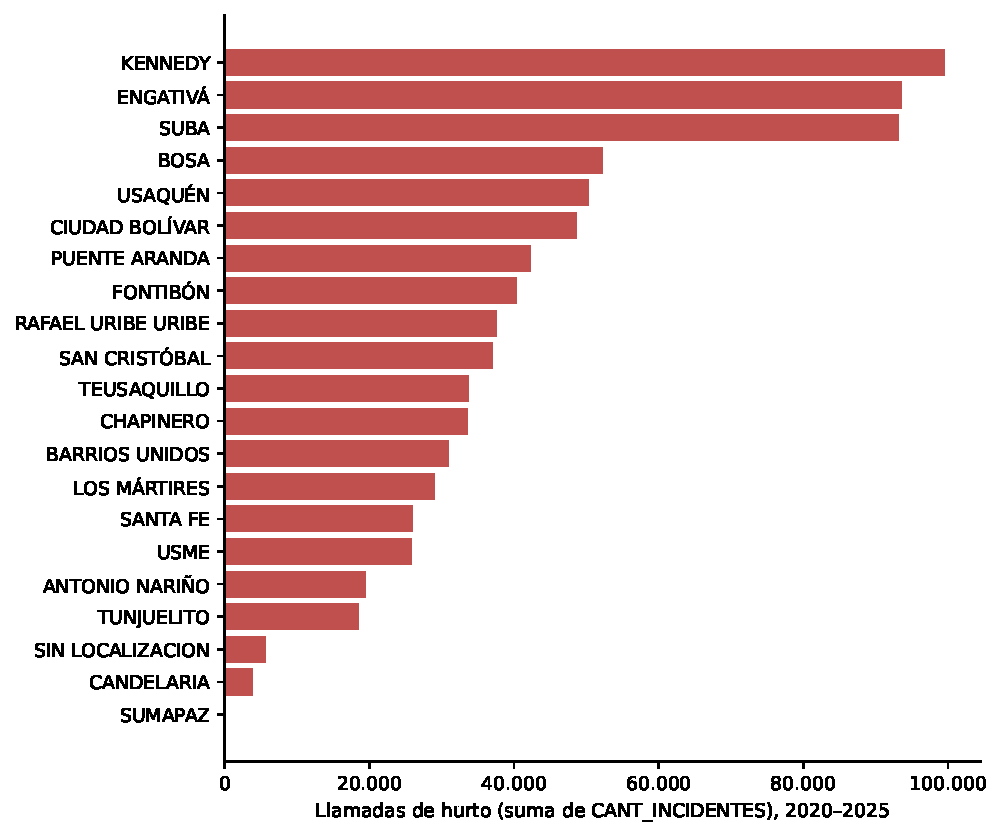
\includegraphics[width=0.78\textwidth]{figuras/linea123_localidad.pdf}}{\fbox{Figura pendiente: \texttt{figuras/linea123\_localidad.pdf}}}
\caption{Llamadas de hurto a la Línea 123 por localidad, 2020--2025 (suma de \texttt{CANT\_INCIDENTES}). Fuente: \texttt{outputs/informe/linea123\_localidad\_2020\_2025.csv}.}\label{fig:localidad}
\end{figure}

\subsection{Calidad de los datos}

La tabla~\ref{tab:calidad} resume los hallazgos de calidad de la población que usa cada fuente. Lo que la auditoría marca como anomalía no siempre es un error: varias marcas son rasgos de la fuente que se documentan, no se corrigen.

{\small
\setlength{\tabcolsep}{4pt}
\begin{longtable}{@{}>{\raggedright\arraybackslash}p{2.2cm}>{\raggedright\arraybackslash}p{6.6cm}>{\raggedright\arraybackslash}p{6.5cm}@{}}
\caption{Hallazgos de calidad y tratamiento previsto.}\label{tab:calidad}\\
\toprule
\textbf{Fuente} & \textbf{Hallazgo} & \textbf{Tratamiento} \\
\midrule
\endfirsthead
\toprule
\textbf{Fuente} & \textbf{Hallazgo} & \textbf{Tratamiento} \\
\midrule
\endhead
\bottomrule
\endfoot
Policía & 713.344 filas idénticas a otra, por falta de identificador & No deduplicar; controlar con el agregado diario \\
\addlinespace
Policía & Nulos: 622 en género (0,08\,\%) y 392 en grupo de edad (0,05\,\%); ninguno en fecha ni en arma & No imputar; tratar el nulo como categoría «no reportado» \\
\addlinespace
Policía & Caída abrupta en noviembre y diciembre de 2025: 5.416 y 5.700 víctimas, frente a 12.228 en octubre. Las mismas cifras aparecen en el agregado de MinDefensa y en los cuadros de salida validados de la Policía, y el hurto a residencias y a comercio de Bogotá cae en los mismos meses & Causa no establecida (issue \#86). Hasta aclararla, esos meses no se usan para evaluar modelos y no se interpretan como un descenso real \\
\addlinespace
Fiscalía & 3.661 filas repetidas, de 3.094 procesos con varios delitos & Contar filas o procesos según el análisis, declarándolo \\
\addlinespace
Fiscalía & 767 filas del total descargado sin fecha del hecho & Quedan fuera del periodo; no se imputan \\
\addlinespace
Fiscalía & Modalidad no identificable en el 94,2\,\% de las filas no excluibles & Citar como hurto en todas sus modalidades \\
\addlinespace
Línea 123 & \texttt{ID} repetido en 166 filas de hurto & No usar \texttt{ID} como clave \\
\addlinespace
Línea 123 & Valores sin ubicación en localidad y UPZ & Separarlos antes de cualquier análisis territorial \\
\end{longtable}
}

\subsection{Cobertura temporal}

La figura~\ref{fig:series} compara las series mensuales de las tres fuentes, cada una en su unidad. Las tres caen en abril de 2020, durante el aislamiento obligatorio, y suben hasta 2022--2023. El tramo de 2018--2019 aparece solo como contexto: para la Policía corresponde al agregado de MinDefensa, porque no hay registros individuales de esos años. La caída de la Policía en noviembre y diciembre de 2025 es la anomalía señalada en la tabla~\ref{tab:calidad}; la Fiscalía también baja en noviembre, de 18.687 a 10.505 filas, pero se recupera en diciembre. Las tres series se comparan en tendencia, no en magnitud: sus unidades son distintas y sus valores no se suman.

\begin{figure}[H]
\centering
\IfFileExists{figuras/series_mensuales_fuentes.pdf}{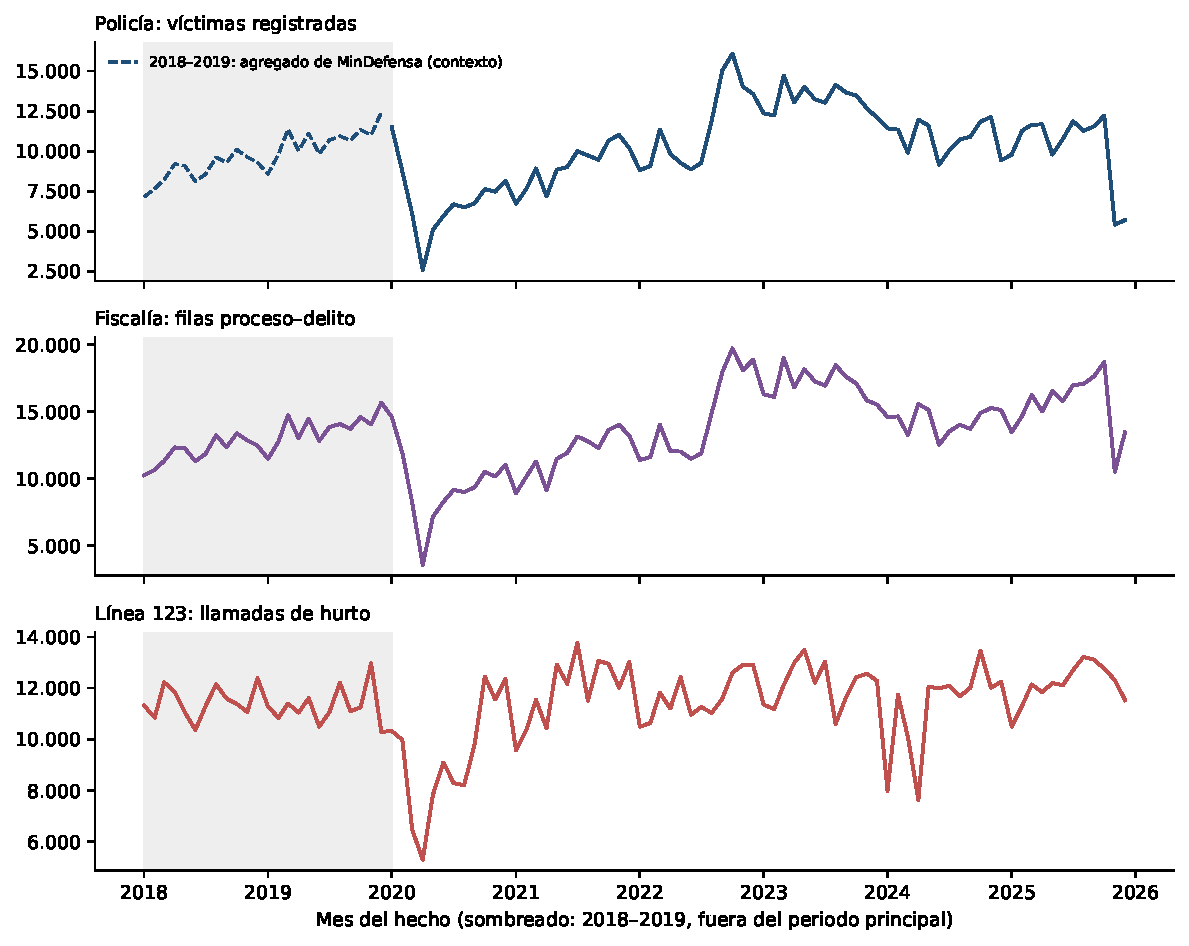
\includegraphics[width=\textwidth]{figuras/series_mensuales_fuentes.pdf}}{\fbox{Figura pendiente: \texttt{figuras/series\_mensuales\_fuentes.pdf}}}
\caption{Series mensuales de las tres fuentes, cada una en su propia unidad. Fuente: \texttt{outputs/informe/series\_mensuales\_fuentes.csv}.}\label{fig:series}
\end{figure}

\subsection{Unidades de observación y posibilidades de integración}

Las tres fuentes describen fenómenos relacionados, pero cada fila representa algo distinto. La tabla~\ref{tab:compatibilidad} resume qué es una fila en cada fuente y con qué resolución temporal y territorial se publica. Las cifras de Línea 123 y Fiscalía provienen de \texttt{outputs/auditoria/}, y las de la Policía, de la auditoría de los seis archivos anuales (\texttt{outputs/auditoria\_policia/}).

{\small
\setlength{\tabcolsep}{4pt}
\begin{longtable}{@{}>{\raggedright\arraybackslash}p{2.6cm}>{\raggedright\arraybackslash}p{4.2cm}>{\raggedright\arraybackslash}p{4.0cm}>{\raggedright\arraybackslash}p{4.2cm}@{}}
\caption{Unidad de observación y granularidad de las fuentes.}\label{tab:compatibilidad}\\
\toprule
\textbf{Característica} & \textbf{Línea 123} & \textbf{Policía Nacional (registro)} & \textbf{Fiscalía (Procesos V3)} \\
\midrule
\endfirsthead
\toprule
\textbf{Característica} & \textbf{Línea 123} & \textbf{Policía Nacional (registro)} & \textbf{Fiscalía (Procesos V3)} \\
\midrule
\endhead
\bottomrule
\endfoot
Qué es una fila & Un agregado de llamadas procedentes por año, mes, localidad, UPZ y tipo de incidente & Un registro con \texttt{CANTIDAD} = 1 que trae el género y el grupo de edad de una persona, es decir, una víctima & Un par proceso--delito (noticia criminal); un mismo proceso puede ocupar varias filas \\
\addlinespace
Medida de conteo & Suma de \texttt{CANT\_INCIDENTES}, no número de filas: 25.144 filas de hurto suman 1.094.313 llamadas (2018--2025) & Número de filas, igual a la suma de \texttt{CANTIDAD}: 741.986 en 2020--2025 & Filas o procesos únicos: 1.300.703 filas y 1.297.042 procesos (2018--2025) \\
\addlinespace
Resolución temporal & Año y mes & Fecha diaria del hecho & Año y mes del hecho (767 filas del total descargado no lo traen); también año y mes de creación del proceso \\
\addlinespace
Resolución territorial & 20 localidades y 116 UPZ, más valores sin ubicación («SIN LOCALIZACION», «SIN UPZ \ldots» y «-»), que suman 121.254 filas de UPZ & Municipio (código DANE); sin localidad ni barrio & Municipio (todo 11001), zona urbana o rural y seccional; sin localidad \\
\addlinespace
Definición de hurto & Tipos de detalle que contienen «hurto»; uno cambia de nombre en 2019 y se homologa por código & \texttt{DELITOS} = «(05022) Hurto a personas» & Capítulo «Del Hurto»: incluye todas las modalidades (personas, automotores, residencias, etc.) \\
\addlinespace
Identificador & \texttt{ID}, no único: 2.633 identificadores repetidos en el archivo completo y 166 en las filas de hurto 2018--2025 & Sin identificador & \texttt{proceso\_anonimizado} \\
\addlinespace
Qué mide & Demanda ciudadana de atención (llamadas) & Hechos denunciados o conocidos por la Policía & Respuesta judicial (procesos abiertos) \\
\end{longtable}
}

\subsubsection{Llaves de integración}

\begin{itemize}
  \item \textbf{Mes $\times$ Bogotá.} Es la única resolución que comparten las tres fuentes: Línea 123 y Fiscalía publican año y mes, y la Policía puede agregarse de día a mes. Sobre esta llave se construirán series paralelas, una por fuente, para comparar tendencias y estudiar desfases (por ejemplo, entre la llamada, el registro policial y la apertura del proceso).
  \item \textbf{Mes $\times$ localidad.} Solo está disponible en Línea 123, así que los análisis territoriales por localidad o UPZ se harán únicamente con esa fuente y no se contrastarán con las otras dos.
  \item \textbf{Día $\times$ Bogotá.} Solo está disponible en la Policía. Permite estudiar estacionalidad semanal y festivos, sin contraparte en las demás fuentes.
\end{itemize}

\subsubsection{Cruces no válidos}

\begin{itemize}
  \item \textbf{Sumar filas o conteos de fuentes distintas.} Una misma situación puede generar una llamada, un registro policial y un proceso, de modo que la suma contaría varias veces el mismo hecho. Tampoco se suman entre fuentes para alcanzar el requisito de 500.000 registros.
  \item \textbf{Enlazar registros individuales.} No hay un identificador común. La Policía no publica identificador y las fuentes no comparten ubicación precisa ni hora, así que no es posible quitar duplicados registro a registro, como en los estudios con microdatos georreferenciados.
  \item \textbf{Comparar territorios sin equivalencia.} Por ejemplo, la distribución por localidad de Línea 123 con el total de la ciudad de las otras fuentes.
  \item \textbf{Equiparar «hurto» entre fuentes sin homologar.} El capítulo «Del Hurto» de la Fiscalía incluye modalidades que no son hurto a personas, y las categorías de Línea 123 son tipificaciones operativas de la llamada.
  \item \textbf{Usar la fecha de creación del proceso como fecha del hecho,} o datos que no estarían disponibles al momento de predecir. Los registros judiciales de un mes pueden completarse meses después, así que su uso como predictor exigirá controlar ese rezago.
\end{itemize}

\subsection{Variable objetivo y conjunto de modelamiento}\label{sec:objetivo}

La variable objetivo es el \textbf{número diario de víctimas de hurto a personas registradas por la Policía Nacional en Bogotá}. Se obtiene contando, para cada fecha del hecho, las filas del registro que pasan los filtros de la tabla~\ref{tab:embudo}. El resultado es una serie de 2.192 días, del 1 de enero de 2020 al 31 de diciembre de 2025, que suma las 741.986 víctimas. Ningún día queda vacío, así que no hay que imputar valores. La tabla~\ref{tab:serie} resume la serie y la figura~\ref{fig:serie} la muestra.

\begin{table}[H]
\centering
\caption{Estadísticas descriptivas de la serie diaria objetivo, 2020--2025.}\label{tab:serie}
\begin{tabular}{@{}lr@{}}
\toprule
\textbf{Estadístico} & \textbf{Valor} \\
\midrule
Días (observaciones del conjunto de modelamiento) & 2.192 \\
Días sin registros & 0 \\
Media de víctimas por día & 338,50 \\
Mediana & 337 \\
Desviación estándar & 115,61 \\
Mínimo & 25 (22 de marzo de 2020) \\
Máximo & 718 (23 de septiembre de 2022) \\
Media del día con más víctimas (viernes) & 398,22 \\
Media del día con menos víctimas (domingo) & 242,29 \\
\bottomrule
\end{tabular}
\end{table}

\begin{figure}[H]
\centering
\IfFileExists{figuras/serie_diaria_policia.pdf}{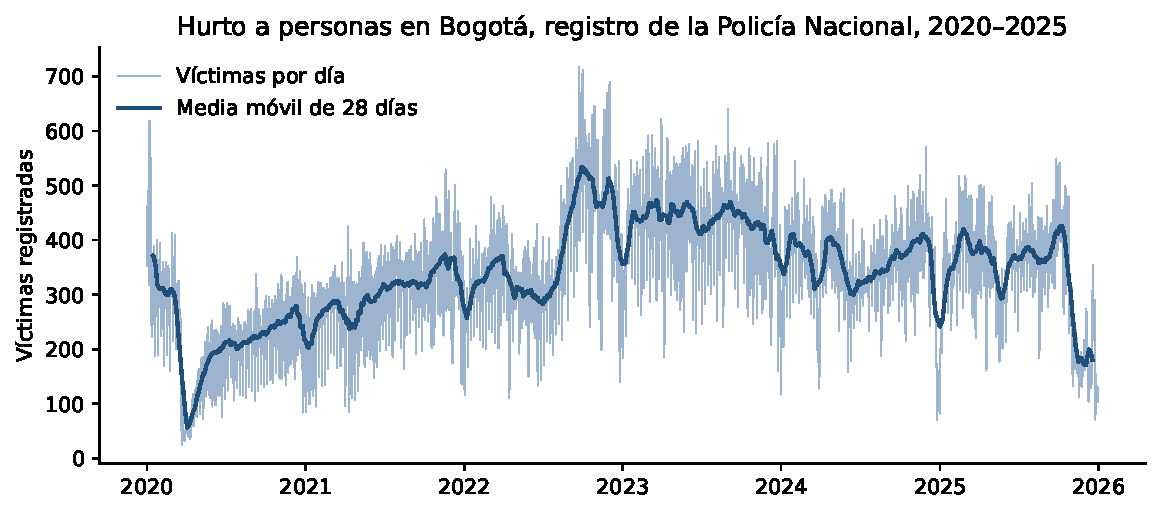
\includegraphics[width=\textwidth]{figuras/serie_diaria_policia.pdf}}{\fbox{Figura pendiente: \texttt{figuras/serie\_diaria\_policia.pdf}}}
\caption{Víctimas diarias de hurto a personas registradas en Bogotá y media móvil de 28 días. Fuente: \texttt{outputs/serie\_objetivo/serie\_diaria\_policia.csv}.}\label{fig:serie}
\end{figure}

La serie muestra cuatro rasgos que el modelamiento deberá tener en cuenta:
\begin{itemize}
  \item un mínimo durante el aislamiento obligatorio de 2020;
  \item una recuperación hasta un máximo en el segundo semestre de 2022;
  \item una estacionalidad semanal marcada, con más registros de martes a sábado que el domingo y el lunes;
  \item la caída de noviembre y diciembre de 2025 descrita en la tabla~\ref{tab:calidad}.
\end{itemize}

Las demás fuentes solo podrán entrar al modelo como variables explicativas si están disponibles antes del día que se pronostica y tienen una justificación metodológica. La Línea 123 y la Fiscalía publican por mes y con rezago, así que su uso en un pronóstico diario exigirá rezagos de al menos un mes. Se evaluará en la segunda entrega.

El pronóstico es para el total de la ciudad. Un pronóstico por localidad no es viable con esta fuente, porque el registro no identifica la localidad.

\subsection{Variables derivadas previstas}

En la segunda entrega se construirán, sobre la serie diaria, variables de calendario (año, mes, día de la semana y festivos), rezagos y estadísticas móviles calculadas solo con observaciones pasadas. Las series de la Línea 123 y de la Fiscalía solo se usarán con el rezago con que estarían disponibles al momento de pronosticar, para evitar filtrar información futura.

Estas variables son propuestas metodológicas, no campos existentes en la base original. Su utilidad real se comprobará mediante el análisis exploratorio y la evaluación de modelos.

\subsection{Criterios previstos de calidad de datos}

Durante el preprocesamiento se comprobarán: \textit{completitud} (nulos y continuidad de fechas), \textit{unicidad} (filas repetidas por fecha y municipio), \textit{validez} (conteos no negativos y formatos), \textit{consistencia territorial} (códigos y nombres), \textit{valores atípicos} (picos o caídas de la serie), y \textit{comparabilidad} (cambios de registro y revisiones de cifras). Los valores extremos no se eliminarán automáticamente, pues pueden corresponder a hechos o circunstancias reales.

También se analizarán localidades ausentes o categorías sin ubicación en las fuentes que las incorporen. Los registros pueden estar afectados por subdenuncia y cambios administrativos \citep{riascos2023}; por ello, las predicciones se interpretarán como proyecciones de conteos registrados y no de la totalidad de eventos ocurridos.

\subsection{Análisis y productos previstos para las siguientes entregas}

La segunda entrega profundizará el análisis exploratorio de la serie objetivo (tendencia, estacionalidad y valores atípicos) y la comparación de tendencias entre fuentes. La tercera comparará modelos de pronóstico de la serie diaria con una línea base estacional ingenua, como repetir el valor del mismo día de la semana anterior, y alternativas como SARIMA, Random Forest y XGBoost.

La evaluación empleará una separación cronológica de entrenamiento y prueba, evitando mezclar observaciones futuras en el entrenamiento. Se considerarán métricas como error absoluto medio (MAE) y raíz del error cuadrático medio (RMSE). Esta sección establece el plan de análisis; \textbf{no presenta preprocesamiento ejecutado, modelos entrenados ni resultados predictivos}, pues estos corresponden a las siguientes entregas.

\subsection{Consideraciones éticas y limitaciones}

El proyecto utilizará fuentes públicas anonimizadas y no elaborará perfiles individuales. La identificación de zonas con mayores conteos no implica que sus habitantes sean responsables de los delitos. Las diferencias territoriales pueden reflejar, entre otros factores, densidad de población, actividades económicas, población flotante, subregistro o calidad de localización. Por tanto, se evitarán conclusiones causales o estigmatizantes y se documentarán los límites de extrapolación de los modelos.
               % Juan Diego

% Secciones de la segunda entrega, a cargo de Sara (#30, #34, #38). Cada una va en su
% archivo de secciones/ y se activa quitando el % cuando exista:
% \input{secciones/05_preprocesamiento}
% \input{secciones/06_analisis_exploratorio}
% \input{secciones/07_metodologia}

% Secciones de la tercera entrega:
% \input{secciones/08_implementacion}
% \input{secciones/09_resultados}
% \input{secciones/10_interpretacion}
% \input{secciones/11_conclusiones}

% Referencias · Se incluye desde informe.tex.
\begin{thebibliography}{}
% Formato APA 7, adaptación en español: «y» entre autores, «s. f.», «Recuperado el ... de».
% Orden alfabético por primer autor. Etiqueta natbib: [cita corta(año)].
% Verificación de cada referencia: docs/verificacion_referencias.md (issue #24).

\bibitem[Campo~Agredo(2017)]{campo2017}
Campo Agredo, C. A. (2017). \emph{Desarrollo de modelos de predicción sobre el hurto a personas en Bogotá a partir del análisis y aplicación de algoritmos en base de datos} [Trabajo de grado de pregrado, Universidad de los Andes]. Repositorio Institucional Séneca. \url{https://hdl.handle.net/1992/50785}

\bibitem[{Fiscalía General de la Nación}(2026)]{fiscalia}
Fiscalía General de la Nación. (2026). \emph{Procesos Fiscalía V3} [Conjunto de datos; corte del 31 de octubre de 2026]. Portal de Datos Abiertos de Colombia. Recuperado el 11 de noviembre de 2026, de \url{https://www.datos.gov.co/d/dbdv-iihs}

\bibitem[Fonseca~Vásquez(2019)]{fonseca2019}
Fonseca Vásquez, A. R. (2019). \emph{Análisis espacial del hurto a personas para la toma de decisiones del Comando de Atención Inmediata (CAI) en la localidad de Los Mártires Bogotá D. C. entre los años 2017--2018} [Trabajo de especialización, Universidad Militar Nueva Granada]. Repositorio Institucional UMNG. \url{https://repository.umng.edu.co/server/api/core/bitstreams/2e3a1b76-45f4-4348-82e1-ace03d817513/content}

\bibitem[Garzón~Acosta(2025)]{garzon2025}
Garzón Acosta, J. J. (2025). \emph{Modelos de predicción del hurto a personas en Bogotá D. C. (2015--2024): Un enfoque comparativo entre MCE y VECM} [Trabajo de especialización, Fundación Universitaria Los Libertadores]. Repositorio Institucional Los Libertadores. \url{https://repository.libertadores.edu.co/bitstreams/45b1a97c-3c66-4beb-988a-95e7dfb9c14b/download}

\bibitem[Martínez~Chitiva(2025)]{martinez2025}
Martínez Chitiva, A. V. (2025). \emph{Análisis espacio-temporal para caracterización, predicción y mitigación del hurto a personas en Bogotá} [Tesis de maestría, Universidad de Manizales]. Repositorio Institucional RIDUM. \url{https://ridum.umanizales.edu.co/handle/20.500.12746/7648}

\bibitem[{Policía Nacional de Colombia}(2026)]{policia}
% Recurso usado (D-01, issue #18): archivos anuales 2020--2025 a nivel de registro.
Policía Nacional de Colombia. (2026). \emph{Información de delitos a nivel de registro} [Conjunto de datos; archivos anuales 2020--2025]. Dirección de Investigación Criminal e INTERPOL. Recuperado el 11 de noviembre de 2026, de \url{https://www.policia.gov.co/estadistica-delictiva}

\bibitem[Provost y Fawcett(2013)]{provost2013}
Provost, F., y Fawcett, T. (2013). \emph{Data science for business: What you need to know about data mining and data-analytic thinking}. O'Reilly Media.

\bibitem[Riascos et~al.(2020)]{riascos2020}
% Número confirmado (issue #24): el listado oficial de la Escuela de Gobierno la presenta como
% «Nota de política No. 38». El «34» de los metadatos del PDF es el nombre del archivo de diseño.
Riascos, A. J., Dulce, M., Moreno, J. S., y Gómez, F. (2020). \emph{Prediciendo el crimen en Bogotá} (Nota de Política n.\textsuperscript{o}~38). Escuela de Gobierno Alberto Lleras Camargo, Universidad de los Andes. \url{https://gobierno.uniandes.edu.co/wp-content/uploads/NP-38.pdf}

\bibitem[Riascos~Villegas et~al.(2023)]{riascos2023}
Riascos Villegas, Á. J., Ñungo, J. S., Gómez Tobón, L., Dulce Rubio, M., y Gómez, F. (2023). Modelling underreported spatio-temporal crime events. \emph{PLOS ONE}, \emph{18}(7), Artículo e0287776. \url{https://doi.org/10.1371/journal.pone.0287776}

\bibitem[{Secretaría Distrital de Seguridad, Convivencia y Justicia}(2026)]{linea123}
Secretaría Distrital de Seguridad, Convivencia y Justicia. (2026). \emph{Llamadas tramitadas C4 Bogotá NUSE Línea 123, enero 2015 -- septiembre 2026} [Conjunto de datos]. Datos Abiertos Bogotá. Recuperado el 11 de noviembre de 2026, de \url{https://datosabiertos.bogota.gov.co/dataset/incidentes}

\bibitem[Urcuqui et~al.(2020)]{urcuqui2020}
Urcuqui, C., Moreno, J., Montenegro, C., Riascos, A., y Dulce, M. (2020). Accuracy and fairness in a conditional generative adversarial model of crime prediction. En \emph{2020 7th International Conference on Behavioural and Social Computing (BESC)} (pp. 1--6). IEEE. \url{https://doi.org/10.1109/BESC51023.2020.9348315}

\end{thebibliography}


\clearpage
\appendix
% Apéndices, Juan Diego (#51) · Se incluye desde informe.tex después de \appendix.
% Fuentes de cada tabla:
%   ap:diccionario  docs/DICCIONARIO_DATOS.md (secciones 2 a 4)
%   ap:archivos     outputs/auditoria/resumen_archivos.csv, outputs/auditoria_policia/resumen_archivos.csv
%                   y las fechas de descarga de data/README.md
%   ap:localidad    outputs/informe/linea123_localidad_2020_2025.csv

\section{Diccionario de datos}\label{ap:diccionario}

Este apéndice resume las variables de las fuentes complementarias y del agregado de control. Las del registro de la Policía están en la tabla~\ref{tab:variables-policia}. El diccionario completo, con el tipo, el número de valores distintos y el nombre original de cada columna, está en \texttt{docs/DICCIONARIO\_\allowbreak{}DATOS.md}. Las definiciones de Fiscalía siguen la ficha oficial del conjunto \citep{fiscalia}.

La columna \emph{Uso} indica el papel previsto en el proyecto: \emph{objetivo}, \emph{predictora}, \emph{filtro}, \emph{trazabilidad}, \emph{descriptiva} (se analiza pero no entra en el modelo) o \emph{no se usa}.

{\small
\begin{longtable}{@{}>{\raggedright\arraybackslash}p{4.2cm}>{\raggedright\arraybackslash}p{8.6cm}>{\raggedright\arraybackslash}p{2.2cm}@{}}
\caption{Variables del agregado diario de MinDefensa (una fila por día y municipio).}\label{tab:dic-agregado}\\
\toprule
\textbf{Variable} & \textbf{Descripción} & \textbf{Uso} \\
\midrule
\endhead
\texttt{fecha\_\allowbreak{}hecho} & Fecha del hecho; un valor por día del periodo & trazabilidad \\
\texttt{cantidad} & Número de hurtos registrados ese día, no una fila por hecho. Suma 975.793 en 2018--2025 & trazabilidad \\
\texttt{cod\_\allowbreak{}muni} & Código DANE del municipio; 11001 tras el filtro & filtro \\
\texttt{municipio}, \texttt{departamento}, \texttt{cod\_\allowbreak{}depto} & Constantes tras el filtro de Bogotá & no se usa \\
\bottomrule
\end{longtable}

\begin{longtable}{@{}>{\raggedright\arraybackslash}p{4.2cm}>{\raggedright\arraybackslash}p{8.6cm}>{\raggedright\arraybackslash}p{2.2cm}@{}}
\caption{Variables de la Línea 123 (una fila por año, mes, localidad, UPZ y tipo de incidente).}\label{tab:dic-linea123}\\
\toprule
\textbf{Variable} & \textbf{Descripción} & \textbf{Uso} \\
\midrule
\endfirsthead
\multicolumn{3}{@{}l}{\emph{Tabla~\ref{tab:dic-linea123} (continuación)}}\\
\toprule
\textbf{Variable} & \textbf{Descripción} & \textbf{Uso} \\
\midrule
\endhead
\texttt{cant\_\allowbreak{}incidentes} & Número de llamadas tramitadas del grupo, no de hechos. Las 25.144 filas de hurto de 2018--2025 suman 1.094.313 & trazabilidad \\
\texttt{anio} & Año del incidente; el archivo cubre 2015--2026 & filtro \\
\texttt{mes} & Mes del incidente, la resolución temporal máxima de la fuente & predictora \\
\texttt{tipo\_\allowbreak{}detalle} & Tipificación operativa de la llamada, no una calificación jurídica. El filtro de hurto busca «HURTO» aquí & filtro \\
\texttt{tipo\_\allowbreak{}incidente} & Categoría superior del incidente & no se usa \\
\texttt{localidad} & Localidad de Bogotá: las 20 localidades más «SIN LOCALIZACION» y «-» & predictora \\
\texttt{cod\_\allowbreak{}localidad} & Código de la localidad & trazabilidad \\
\texttt{upz}, \texttt{cod\_\allowbreak{}upz} & Unidad de planeamiento zonal: 116 UPZ más 9 valores sin ubicación & predictora \\
\texttt{id} & No es único: 2.633 identificadores se repiten en el archivo y 166 en las filas de hurto del periodo. No sirve como clave & no se usa \\
\bottomrule
\end{longtable}

\begin{longtable}{@{}>{\raggedright\arraybackslash}p{4.2cm}>{\raggedright\arraybackslash}p{8.6cm}>{\raggedright\arraybackslash}p{2.2cm}@{}}
\caption{Variables de Procesos Fiscalía V3 (una fila por par proceso--delito).}\label{tab:dic-fiscalia}\\
\toprule
\textbf{Variable} & \textbf{Descripción} & \textbf{Uso} \\
\midrule
\endfirsthead
\multicolumn{3}{@{}l}{\emph{Tabla~\ref{tab:dic-fiscalia} (continuación)}}\\
\toprule
\textbf{Variable} & \textbf{Descripción} & \textbf{Uso} \\
\midrule
\endhead
\texttt{proceso\_\allowbreak{}anonimizado} & Identificador anonimizado del proceso; permite contar procesos distintos frente a filas & trazabilidad \\
\texttt{a\_\allowbreak{}o\_\allowbreak{}hecho}, \texttt{mes\_\allowbreak{}hecho} & Año y mes del hecho. Las 767 filas con mes «Sin Información» no traen año y quedan fuera de 2018--2025 & filtro \\
\texttt{a\_\allowbreak{}o\_\allowbreak{}creacion\_\allowbreak{}proceso}, \texttt{mes\_\allowbreak{}creacion\_\allowbreak{}proceso} & Año y mes de creación del proceso. No es la fecha del hecho: usarla como tal introduce fuga de información & no se usa \\
\texttt{delito} & Tipo penal: artículo, cuantía y agravación. No codifica la víctima, así que no aísla el hurto a personas (tabla~\ref{tab:fiscalia}) & descriptiva \\
\texttt{capitulo\_\allowbreak{}delito} & «Del Hurto» tras el filtro; incluye todas las modalidades & filtro \\
\texttt{titulo\_\allowbreak{}delito} & «Delitos Contra El Patrimonio Economico»; constante tras el filtro & no se usa \\
\texttt{grado\_\allowbreak{}delito} & Distingue la tentativa del delito consumado. En 2018--2025: Ninguno (1.209.762), Agravado (80.678), Tentativa (6.005) y Tentativa/Agravado (4.258) & descriptiva \\
\texttt{estado} & Situación de la investigación «al momento de la consulta»: Activo o Inactivo. Es fuga de información & no se usa \\
\texttt{etapa} & Macroetapa procesal: Indagación, Investigación, Juicio y Ejecución de Penas. Depende del tiempo transcurrido; es fuga de información & no se usa \\
\texttt{tipo\_\allowbreak{}noticia} & Fuente por la que se inicia la investigación, por ejemplo denuncia, de oficio o querella & descriptiva \\
\texttt{dir\_\allowbreak{}hecho\_\allowbreak{}rural\_\allowbreak{}urbana} & Zona del hecho; incluye «Sin Información» & descriptiva \\
\texttt{seccional} & Dependencia de la Fiscalía asignada, no ubicación del hecho. El 99,89\,\% de las filas de 2018--2025 es la Dirección Seccional de Bogotá & no se usa \\
\texttt{cod\_\allowbreak{}dane\_\allowbreak{}hecho} & 11001 tras el filtro & filtro \\
\texttt{delito\_\allowbreak{}querellable} & Si el delito es querellable; Sí en 114.259 filas & descriptiva \\
\texttt{proceso\_\allowbreak{}conexado} & Si el proceso fue fusionado a otro (art.~51 del CPP); Sí en 4.772 filas & trazabilidad \\
\texttt{proceso\_\allowbreak{}con\_\allowbreak{}conexidad} & Si el proceso recibe información de otros (art.~51 del CPP); Sí en 3.130 filas & trazabilidad \\
\texttt{es\_\allowbreak{}ruptura} & Si hubo ruptura de la unidad procesal (art.~53 del CPP), que genera un nuevo proceso sobre los mismos hechos; Sí en 4.432 filas & trazabilidad \\
\texttt{procedimiento\_\allowbreak{}abreviado} & Si se tramita por el procedimiento abreviado de la Ley 1826 de 2017; Sí en 1.238.967 filas & descriptiva \\
\texttt{tipo\_\allowbreak{}delito} & «Reparto» (conducta principal, 1.289.368 filas) o «Concurso» (adicional, 11.335) & descriptiva \\
\texttt{ley} & Norma procesal: Ley 906 (1.293.313), Ley 1098 (7.364) y Jurisdicción Menores (26) & descriptiva \\
\texttt{deli\_\allowbreak{}id} & Código interno del delito, redundante con \texttt{delito} & no se usa \\
\texttt{trimestre\_\allowbreak{}hecho}, \texttt{trimestre\_\allowbreak{}creacion} & Trimestre, redundante con el mes & no se usa \\
\texttt{pais\_\allowbreak{}hecho}, \texttt{departamento\_\allowbreak{}hecho}, \texttt{municipio\_\allowbreak{}hecho} & Constantes tras el filtro de Bogotá & no se usa \\
\texttt{fecha\_\allowbreak{}corte\_\allowbreak{}datos} & Fecha de corte de la extracción: 31/10/2026 & trazabilidad \\
\bottomrule
\end{longtable}
}

\section{Archivos de origen y su integridad}\label{ap:archivos}

La tabla~\ref{tab:archivos} identifica cada archivo analizado con su fecha de descarga, su número de filas y su huella SHA-256. Un archivo descargado de nuevo con la misma huella es idéntico al usado en el informe. Los portales actualizan los recursos, así que una descarga posterior puede tener otra huella y otras cifras sin que eso sea un error.

Las huellas de la Policía corresponden a los CSV convertidos desde los \texttt{.xlsx} publicados, que es lo que lee la auditoría. El conversor guarda la huella de cada \texttt{.xlsx} de origen en \texttt{data/raw/policia\_\allowbreak{}registro/csv/conversion.json}, fuera del repositorio. El archivo de la Línea 123 se identifica en \texttt{outputs/auditoria/resumen\_\allowbreak{}archivos.csv} con su nombre completo.

{\scriptsize
\begin{longtable}{@{}>{\raggedright\arraybackslash}p{2.4cm}cr>{\ttfamily}l@{}}
\caption{Archivos de origen: fecha de descarga, filas y SHA-256.}\label{tab:archivos}\\
\toprule
\textbf{Archivo} & \textbf{Descarga} & \textbf{Filas} & \normalfont\textbf{SHA-256} \\
\midrule
\endhead
Línea 123, CSV oficial & 2026-11-09 & 1.117.394 & ceeee37729c83adaae6907272457998cc5a60eaf57c14a5ead17c6db2d3a4d61 \\
\texttt{fiscalia\_\allowbreak{}v3\_\allowbreak{}bogota\_\allowbreak{}hurto.csv} & 2026-11-11 & 2.002.177 & e2f30087b82544e448d0c3f9f04eabd760012b2143e2ab2af632e1d81ff8f2ae \\
\texttt{delitos\_\allowbreak{}registro\_\allowbreak{}2020.csv} & 2026-11-11 & 651.206 & aa2f39e87d899929d07daadfeca2480c0300a5bc0a6cfaa16665c1248fce95eb \\
\texttt{delitos\_\allowbreak{}registro\_\allowbreak{}2021.csv} & 2026-11-11 & 792.244 & 952334b45f2c1ae8160686399c67724abc02af8fe5fbe8c0cc8007d48e73e278 \\
\texttt{delitos\_\allowbreak{}registro\_\allowbreak{}2022.csv} & 2026-11-11 & 862.451 & 8e22e2d1f40a3eed0c274fdc17d02e6afde9dff960eb72fc6398994a43d25385 \\
\texttt{delitos\_\allowbreak{}registro\_\allowbreak{}2023.csv} & 2026-11-11 & 917.544 & d5d34adc3e3f9be79919ed9ae9468589150035dda640169927118efab135c615 \\
\texttt{delitos\_\allowbreak{}registro\_\allowbreak{}2024.csv} & 2026-11-11 & 832.475 & 621a8cd32b6d9194299dd5229404bb66318ebf4b66e14b21681cb4fd80d63c64 \\
\texttt{delitos\_\allowbreak{}registro\_\allowbreak{}2025.csv} & 2026-11-11 & 773.950 & e8c80f134bc260693a7f1ce280372259a607bb41614c65c7df13fa43c7eeaff8 \\
\texttt{hurto\_\allowbreak{}bogota.csv} (MinDefensa) & 2026-11-09 & 2.922 & 32cda715025fc89c6d6ce7de9c36fcb8444e877e00ed5d333feffde7a295b8d6 \\
\bottomrule
\end{longtable}
}

Las filas de los archivos de la Policía son las de todo el país, antes de los filtros de la tabla~\ref{tab:embudo}; suman 4.829.870. Las de Fiscalía son las descargadas con el filtro de Bogotá y del capítulo «Del Hurto», antes de restringir el periodo.

\section{Reproducibilidad}\label{ap:reproducibilidad}

El código, los resultados agregados y el informe están en el repositorio \url{https://github.com/SarAlbN1/AD-DelitosBog}. La versión de la primera entrega es la etiqueta \texttt{entrega-1}. Los datos no se publican en el repositorio: se descargan con las instrucciones de \texttt{data/README.md}, y la guía completa está en \texttt{docs/REPRODUCIBILIDAD.md}. Esa guía distingue dos modos:
\begin{itemize}
  \item \textbf{copia congelada:} con los mismos archivos que usó el equipo, deben coincidir las huellas de la tabla~\ref{tab:archivos} y todas las cifras de \texttt{outputs/auditoria/};
  \item \textbf{descarga nueva:} con los datos del día, se reproduce el procedimiento, pero las huellas y las cifras pueden cambiar.
\end{itemize}

Las cifras y figuras de la sección~\ref{sec:datos} se regeneran en este orden:
\begin{enumerate}
  \item \texttt{scripts/policia\_\allowbreak{}registro\_\allowbreak{}a\_\allowbreak{}csv.py} convierte los archivos anuales de la Policía a CSV;
  \item \texttt{scripts/\allowbreak{}auditoria\_\allowbreak{}datasets.py} produce dos carpetas: \texttt{outputs/auditoria/}, con la Línea 123 y Fiscalía, y \texttt{outputs/auditoria\_\allowbreak{}policia/}, con el registro de la Policía y el agregado de MinDefensa;
  \item \texttt{scripts/serie\_\allowbreak{}objetivo\_\allowbreak{}policia.py} construye la serie objetivo en \texttt{outputs/serie\_\allowbreak{}objetivo/};
  \item \texttt{scripts/fiscalia\_\allowbreak{}modalidades.py} y \texttt{scripts/figuras\_\allowbreak{}informe.py} producen las tablas y figuras de \texttt{outputs/informe/}.
\end{enumerate}
Las figuras de \texttt{Informe/figuras/} son copias de las de \texttt{outputs/} y hay que volver a copiarlas si se regeneran.

\section{Tablas complementarias}\label{ap:tablas}

La tabla~\ref{tab:localidad-ap} da los valores de la figura~\ref{fig:localidad}. Las filas son agregados de la fuente y las llamadas son la suma de \texttt{CANT\_\allowbreak{}INCIDENTES}; los porcentajes se calculan sobre las llamadas y, redondeados, suman 99,99.

{\small
\begin{longtable}{@{}lrrr@{}}
\caption{Llamadas de hurto a la Línea 123 por localidad, 2020--2025.}\label{tab:localidad-ap}\\
\toprule
\textbf{Localidad} & \textbf{Filas} & \textbf{Llamadas} & \textbf{\% de llamadas} \\
\midrule
\endhead
Kennedy & 1.872 & 99.525 & 12,12 \\
Engativá & 1.435 & 93.654 & 11,40 \\
Suba & 1.875 & 93.132 & 11,34 \\
Bosa & 864 & 52.210 & 6,36 \\
Usaquén & 1.506 & 50.245 & 6,12 \\
Ciudad Bolívar & 1.277 & 48.636 & 5,92 \\
Puente Aranda & 863 & 42.313 & 5,15 \\
Fontibón & 1.281 & 40.371 & 4,92 \\
Rafael Uribe Uribe & 926 & 37.524 & 4,57 \\
San Cristóbal & 958 & 36.998 & 4,50 \\
Teusaquillo & 1.007 & 33.702 & 4,10 \\
Chapinero & 920 & 33.584 & 4,09 \\
Barrios Unidos & 710 & 30.974 & 3,77 \\
Los Mártires & 432 & 29.033 & 3,53 \\
Santa Fe & 908 & 25.991 & 3,16 \\
Usme & 1.100 & 25.890 & 3,15 \\
Antonio Nariño & 429 & 19.521 & 2,38 \\
Tunjuelito & 431 & 18.446 & 2,25 \\
Sin localización & 195 & 5.683 & 0,69 \\
Candelaria & 264 & 3.834 & 0,47 \\
Sumapaz & 33 & 38 & 0,00 \\
\midrule
\textbf{Total} & \textbf{19.286} & \textbf{821.304} & \textbf{100} \\
\bottomrule
\end{longtable}
}
            % Juan Diego (#51)

\end{document}
